%%%%%%%%%%%%%%%%%%%%%%%%%%%%%%%%%%%%%%%%%%%%%%%%%%%%%%%%%%%%%%%%%%%%%%%%
% Preamble
%%%%%%%%%%%%%%%%%%%%%%%%%%%%%%%%%%%%%%%%%%%%%%%%%%%%%%%%%%%%%%%%%%%%%%%%
\documentclass[12pt]{article}
%
% Packages and other includes
% Pagination
\usepackage[letterpaper, margin=1in]{geometry}
%
% Graphics, floats, tables
\usepackage{graphicx, color, float, array}
\graphicspath{{image/}}
%
% Fonts
\usepackage[T1]{fontenc} % best for Western European languages
\usepackage{lmodern} % Latin Modern instead of CM
\usepackage{textcomp} % required to get special symbols
%
% Math
\usepackage{amsmath, amssymb}
\usepackage{enumerate}
\usepackage{braket}
% 
% Hyperlinks
\usepackage[colorlinks,linkcolor={red},citecolor={blue},
urlcolor={blue}]{hyperref} 
%
% Definitions and settings
% Paragraph indent and spacing
\setlength{\parskip}{0.4\baselineskip}
\setlength{\parindent}{0in}
%
% Math mode version of "r" column type (requires array package)
\newcolumntype{R}{>{$}r<{$}}
% Title, authors, date
\title{\textbf{Lewis Structures and VSEPR Model}}
\date{Nov 13, 2023}

\begin{document}

\maketitle 

Draw the Lewis structure showing the formal charges. At each central atom, determine the
electronic arrangement, and molecular geometry for the following compounds. Include all
resonance structures and show the resonance hybrid structure:

\begin{enumerate}[(a)]
\item CO$_3^{2-}$
  \vspace{1in}
\item SO$_3$
  \vspace{1in}
\item I$_3^-$
  \vspace{1.2in}
\item SF$_5^-$
  \vspace{1.2in}
\item CH$_2$FCH$_2$COOH
  \vspace{1in}
\item XeF$_4$
  \vspace{1in}
\item CHF$_3$
  \vspace{1in}
\item O$_3$
  \vspace{1in}
\item HCCH
  \vspace{1in}
\item CHONH$_2$
  \vspace{1in}
\item PF$_6$
  \vspace{1in}
\end{enumerate}

\newpage

\begin{center}
  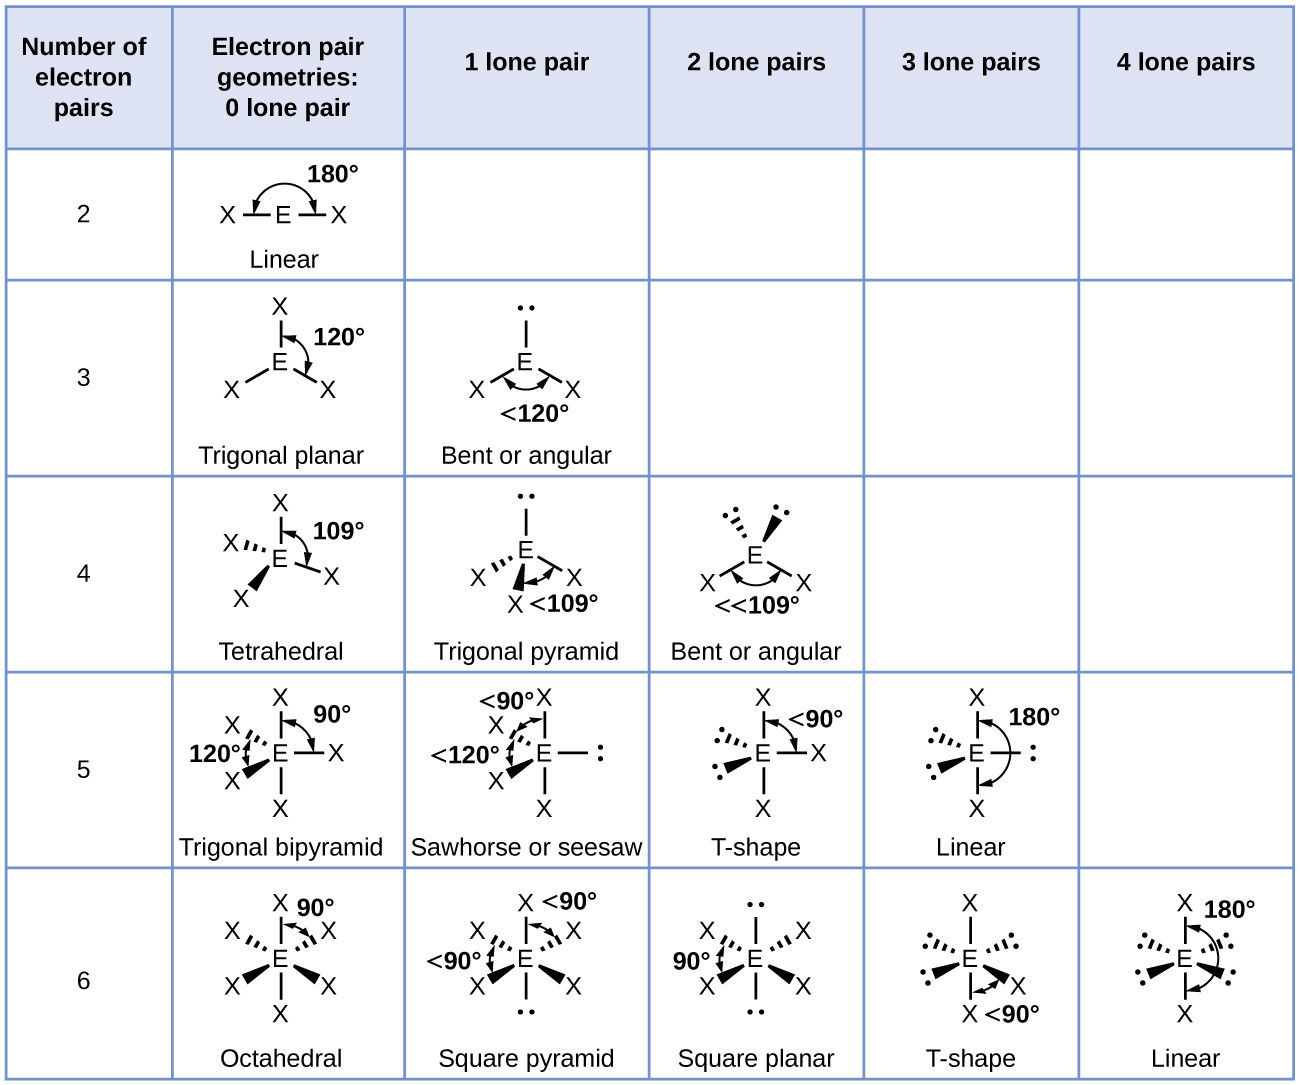
\includegraphics[scale=1]{geo_shape}
\end{center}

\end{document}
